\documentclass[10pt,a4paper]{article}
\usepackage[utf8]{inputenc}
\usepackage[italian]{babel}
\usepackage{amsmath}
\usepackage{amsfonts}
\usepackage{amssymb}
\usepackage{graphicx}
\usepackage[left=2cm,right=2cm,top=2cm,bottom=2cm]{geometry}
\newcommand{\rem}[1]{[\emph{#1}]}

\author{Gruppo AC \\ Federico Belliardo, Giulia Franchi, Francesco Mazzoncini}
\title{Esperienza di Franck-Hertz}
\begin{document}

\maketitle

%Al link http://scipy-cookbook.readthedocs.io/items/SignalSmooth.html è presente una funzione python per eseguire lo smothing i un array 1d di dati, può essere utile per trovare in seguito i massimi locali da associare agli eventi di eccitazione.
%Verificare se sono interspaziati
%Gli elettroni eccitano sempre il primo livello energetico disponibile non arrivano mai ad avere abbastanza energia da eccitare livelli superiori
%Devo guradre i minimi o i massimi?
%Spegare procedura per interpolazione e estrazione di E_A per estrapolazione e calcolo di \lambda
%Acquisizione dati oscilloscopio con il pc

%TODO Ci sono un po' troppe ripetizioni con la scheda dell'esperienza, tutte questi cose preparatorie potrebbero essere saltate e si potrebbe andare direttamente alla descrizione dell'elebaorazione dei dati

\section{Scopo dell'esperienza}
Obiettivo dell'esperienza è dimostrare la struttura discreta dei livelli energetici dell'atomo di neon e di stimarne l'energia di eccitazione mediante lo studio degli effetti dissipativi negli urti anelastici di elettroni su atomi di neon.

\section{Materiale occorrente}

\section{Descrizione esperimento di Franck-Hertz}

\section{Descrizione apparato sperimentale}


\begin{figure}[!htb]
  \centering
  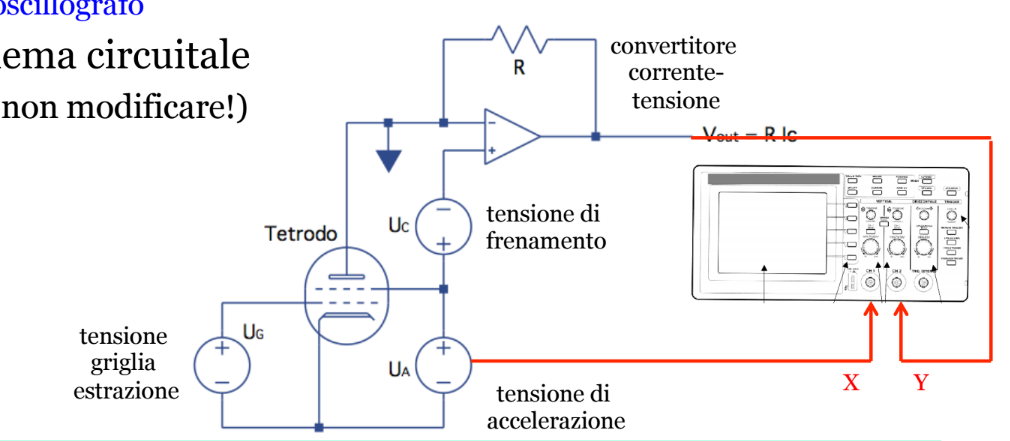
\includegraphics[scale=.5]{circuito.png}
\caption{Schema circuito dell'esperimento e di acquisizione dati.}
\label{circuito}
\end{figure}


\section{Modalità operative}

\section{Osservazioni qualitative}

\section{Raccolta dati ed elaborazione}

%riporto tabelle grafici e fit, interpolazioni per 

\section{Conclusioni}
%Cerco sul manuale quale è la pressione del neon nell'apparecchio e verico che torna con il libero cammino medio fittato








\end{document}


